\section{Wellen}

Die \textbf{Wellengleichung} ist die partielle Differentialgleichung der Form
\begin{empheq}[box=\bluebase]{equation*}
    \frac{\del^2\xi}{\del t^2} - v^2 \frac{\del^2 \xi}{\del x^2} = 0
\end{empheq}
und hat die allgemeine Lösung 
\begin{align*}
    \xi(x,t) = f(x - vt) + g(x+vt)
\end{align*}

Die Auslenkung kann dabei entweder in Ausbreitungsrichtung (Longitudinal) sein, oder senkrecht dazu (transversal). \\
\begin{tabular}{ll}
    \textbf{Transversale Wellen} & \textbf{Longitudinale Wellen}\\
    $v = \sqrt{\frac{S}{\rho}} = \sqrt{\frac{F}{\mu}}$ & $v = \sqrt{\frac{E}{\rho}} = \sqrt{\frac{P}{\rho}}$\\
\end{tabular}\\
$S = \frac{F}{A}$: Zugspannung, $\rho$: Dichte $\mu$: Längendichte, $E = \frac{\sigma}{\epsilon_{\text{el}}}$: Elastizitätsmodul. \\
Für $A$: Fläche, $\sigma = \frac{d F_{\bot}}{d a}$: Normalspannung, $\epsilon_{\text{el}} = \frac{\Delta \ell}{\ell}$

\textbf{Mehrdimensionale Wellen}
Für Wellen im Raum, mit Wellenvektor $\bm{k}$ wird dies zu
\begin{empheq}[box=\bluebase]{align*}
    \frac{\del^2 \bm{\xi}(\bm{r},t)}{\del t^2} - v^2 \Delta \bm{\xi}(\bm{r},t)
\end{empheq}
und nimmt die folgende Form an
\begin{align*}
    \bm{\xi}(\bm{r},t) = \bm{A} e^{i \left(\bm{k \cdot r} - \omega t\right)}
\end{align*}

\textbf{Kugelwellen}
Die Kugelwellengleichung ist gegeben durch
\begin{align*}
    \frac{\del^2 \mathbf{\xi}(\mathbf{x},t)}{\del t^2} - v^2 \left(\frac{\del^2}{\del r^2} + \frac{2}{r} \frac{\del}{\del r}\right) \mathbf{\xi}(\mathbf{x},t) = 0
\end{align*}



\subsection{Energietransport}
Mechanische Wellen transportieren durch ein Medium mit Dichte $\rho$ Energie in zwei Formen. Für transversale Wellen ist dies
\begin{align*}
    \frac{d E_{\text{kin}}}{dV} = \frac{1}{2} \rho \left(\frac{\del \mathbf{\xi}}{\del t}\right)^2 = \frac{d E_{\text{el}}}{dV} =  \frac{1}{2} S \left(\frac{\del \xi}{\del x}\right)^2\\
    \frac{d W}{dV} = \frac{d E_{\text{kin}}}{d V} + \frac{d E_{\text{el}}}{d V} = \rho v^2 \left(\frac{\del \xi}{\del x}\right)^2
\end{align*}
Für Longitudinale Wellen erhält man die Formeln
\begin{align*}
    \frac{d E_{\text{kin}}}{d V} = \frac{1}{2} \rho (\frac{\del \xi}{\del t})^2 = \frac{d E_{\text{el}}}{d V} = \frac{1}{2} E (\frac{\del \xi}{\del x})^2
\end{align*}
Harmonische Wellen der Form $\xi(x,t) = A \cos(k x - \omega t )$ ist die Energiedichte 
\begin{align*}
    \frac{d W}{d V} = \rho \omega^2 A^2 \sin^2(kx -  \omega t)
\end{align*}
und ihre \textbf{mittlere Energiedichte} beträgt
\begin{empheq}[box=\bluebase]{align*}
    \left<\frac{d W}{d V}\right> = \rho \omega^2 A^2 \frac{1}{T} \int_{0}^{T} \sin^2(kx - \omega t) dt = \frac{1}{2} \rho \omega^2 A^2
\end{empheq}

Der \textbf{Poynting-Vektor} misst die Energie, die durch eine Fläche pro Zeit fliesst.

\begin{empheq}[box=\bluebase]{align*}
    \bm{S} = \frac{d^2W}{\Norm{d \vec{a}} dt} \cdot d \hat{\bm{a}}
\end{empheq}
Wobei $\left[S\right] = \frac{\text{J}}{\text{m}^2 \text{s}}\frac{W}{m^2}$. Die \textbf{Intensität} ist dann ihr Absolutbetrag: $I = \abs{S}$  und es gilt
\begin{align*}
    \left<I\right> = \frac{d W}{d V} \cdot v = \frac{1}{2}\rho \omega^2 A^2v = \frac{1}{2}\rho \frac{\omega^3}{k}A^2
\end{align*}


\subsection{Superposition \& Interferenz}
Die Superposition zweier Wellen ist wieder eine Welle.
Ist zum Beispiel $\xi(x,t) = \xi_1(x,t) + \xi_2(x,t)$ die Summe zweier harmonischer Wellen in gleicher Ausbreitungsrichtung aber andere Amplitude und Phase, so erhält man
\begin{align*}
    \xi(x,t) &= A \sin(k x_1 - \omega t) + B \sin(k x_2 -\omega t + \delta)\\
    &= C \sin(\omega t +\phi)
\end{align*}
wobei die Resultierende Amplitude $C$ und die Phasenverschiebung $\phi$ gegeben sind durch
\begin{align*}
    C &= \sqrt{A^2 + B^2 + 2AB \cos\delta}\\
    \phi &= \arccos \frac{A + B \cos \delta}{C} = \arcsin \frac{B \sin \delta}{C}
\end{align*}
Im Spezialfall von $A = B$ erhält man dann
\begin{align*}
    \xi(x,t) = 2A \cos \left[\frac{1}{2}(\delta + k \Delta x)\right] \cos \left[k x_1 - \omega t + \frac{1}{2}(\delta + k \Delta x)\right]
\end{align*}
Im Falle von gleicher Phase und Amplitude, aber unterschiedliche Frequenzen erhält man
\begin{align*}
    \xi(x,t) = 2A \cos \left(\frac{\omega_1 + \omega_2}{2}t\right) \cdot \cos \left(\frac{\omega_1 - \omega_2}{2}t\right)
\end{align*}

\subsection{Reflexion \& Transmission}
Tritt eine Welle von einem Medium mit Geschwindigkeit $v_1$ in ein anderes Medium mit Geschwindigkeit $v_2$ über, so entsteht eine reflexierte und eine transmittierte Welle. Für
\begin{align*}
    \alpha := \frac{\kappa_2}{\kappa_1} = \frac{v_1}{v_2}  = \sqrt{\frac{S_1 \rho_2}{S_2\rho_1}} = \sqrt{\frac{F_1 \mu_2}{F_2 \mu_1}}
\end{align*}
und eine harmonische eintretende Welle $\xi_A(x,t)$ sind die Resultierenden Wellen      
\begin{align*}
    \xi_A(x,t) = A \cdot e^{i(k_1x - \omega t)}\\\xi_R(x,t) = R \cdot e^{i(-k_1x-\omega t + \delta_R)}\\\xi_T(x,t) = T \cdot e^{i(k_2 x - \omega t)}
\end{align*}

\begin{itemize}
    \item[$\alpha > 1$]     Übertritt in härteres Medium.
    \begin{empheq}[box=\bluebase]{align*}
        &\delta_R = \pi, \quad R = \frac{\alpha - 1}{\alpha+1}A, \quad T = \frac{2A}{\alpha + 1} \\
        \lim_{\alpha \to \infty}:\  &\delta_R = \pi \quad R = A \quad T = 0
    \end{empheq}
    \item[$\alpha < 1$]     Übertritt ins weichere Medium.  
    \begin{empheq}[box=\bluebase]{align*}
        &\delta_R = 0, \quad R = \frac{1 - \alpha}{1 + \alpha} \quad T = \frac{2A}{1 + \alpha}\\
        \lim_{\alpha \to 0}: &\delta_R = 0, R = A, \quad \bm{T = 0} \text{ Vakuum!}
    \end{empheq}
\end{itemize}
\begin{figure}[h]
    \centering
    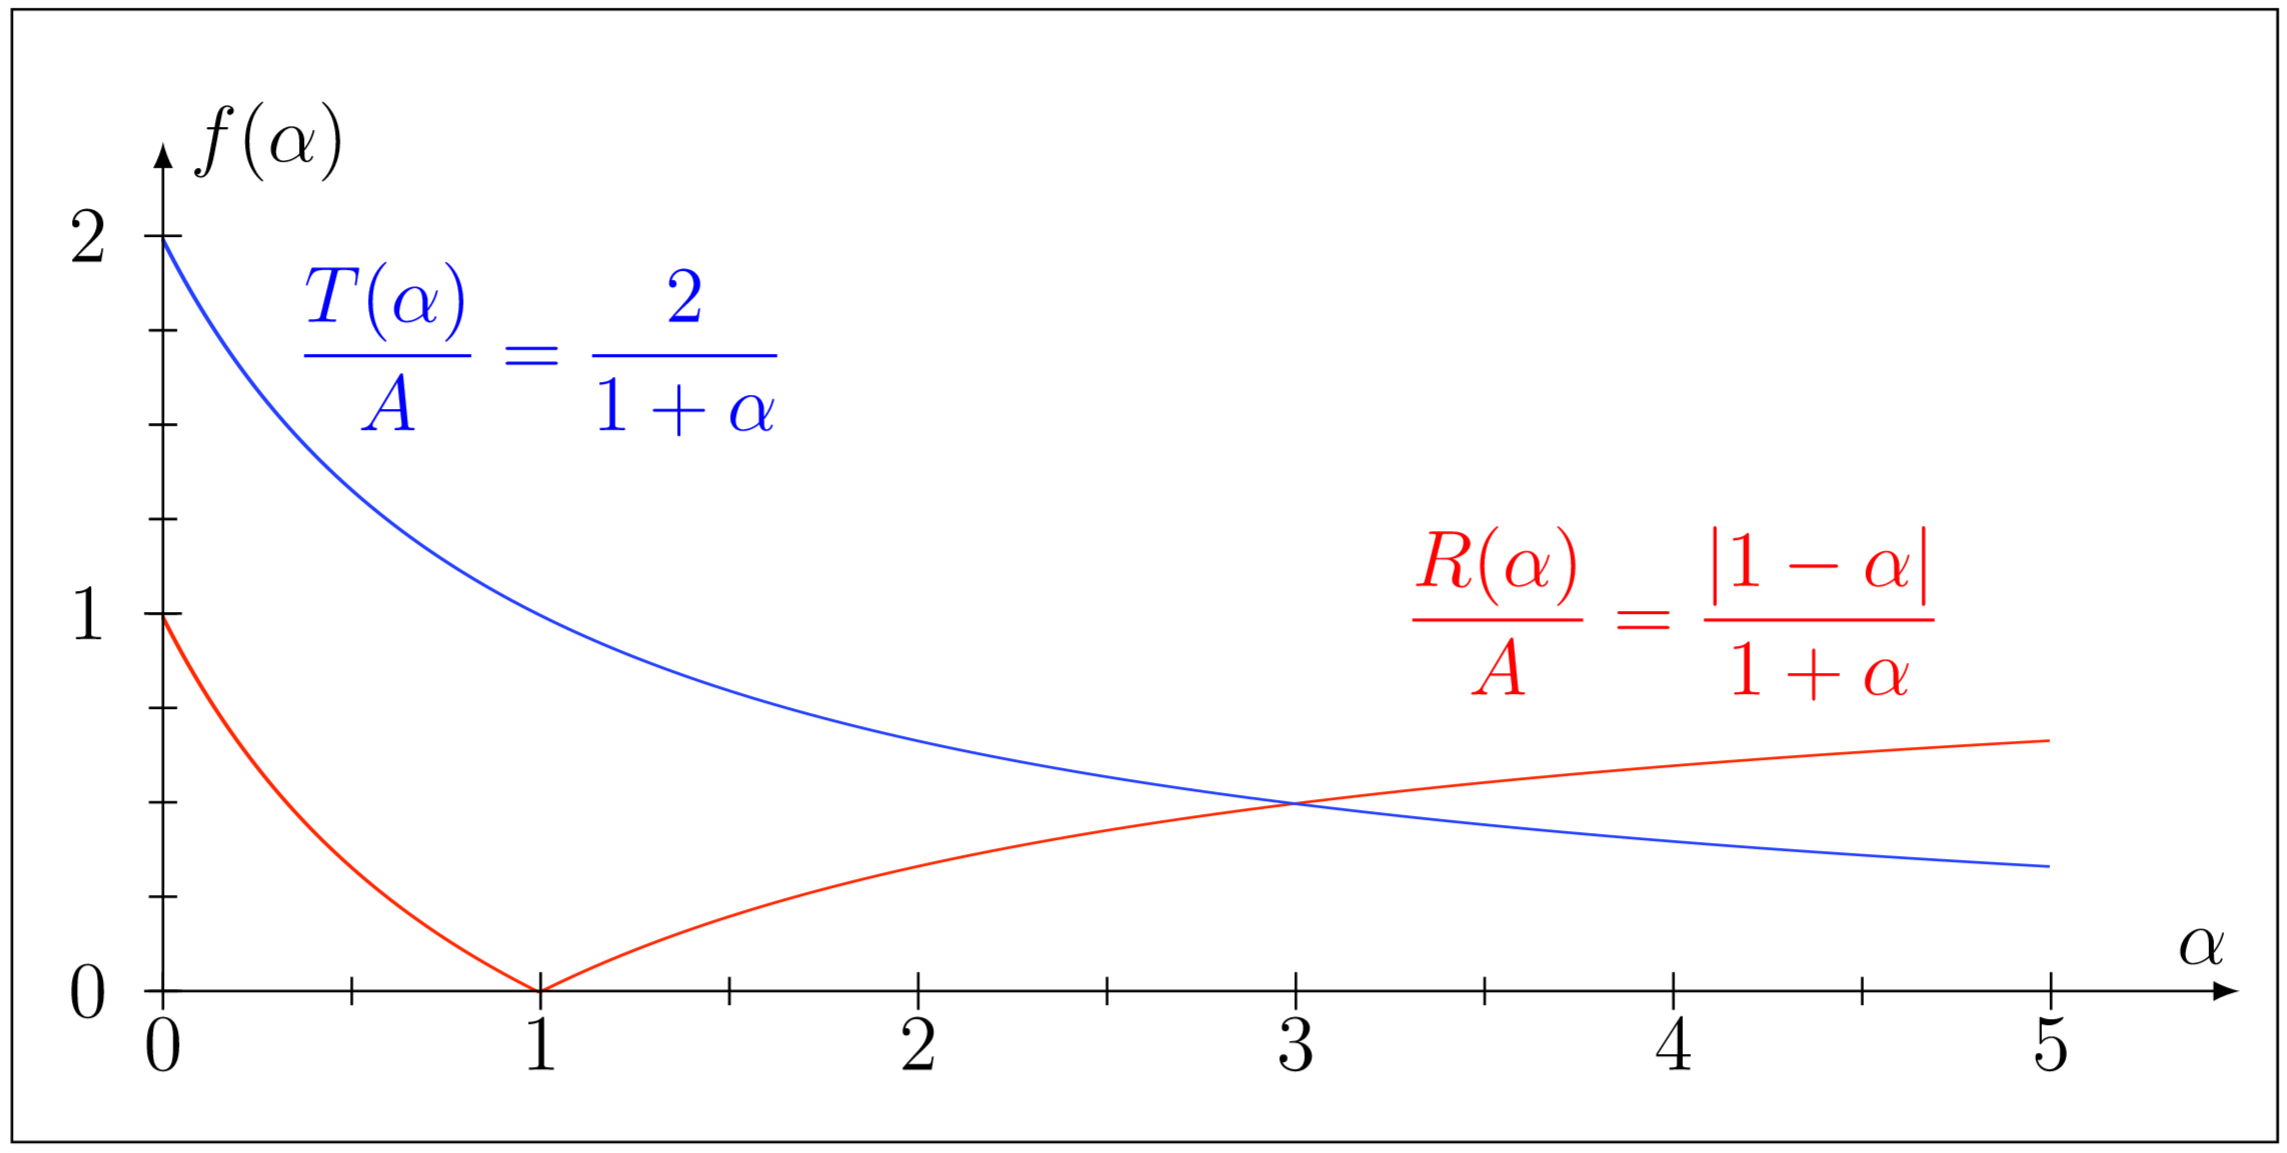
\includegraphics[width =  0.35\textwidth]{images/Reflexion-Transmission}
    \caption{Amplituden der reflektierten und transmittierten Wellen}
\end{figure}

\subsection{Stehende Wellen}
Bei der Reflexion erhalten wir durch die Superposition von Eingehender und Reflektierter Welle die Resultierende Welle in Form von
\begin{empheq}[box=\bluebase]{align*}
    \xi(x,t) = \left\{ \begin{array}{rcl}
        2A \sin(kx)\sin(\omega t), &\text{für}& \alpha \gg 1 \delta_R = \pi \text{ (hartes Ende)}\\
        2A \cos(kx)\cos(\omega t) &\text{für}&  \alpha = 0, \delta_R = 0 \text{ (loses Ende)}
    \end{array} \right.
\end{empheq}

Für \emph{fest eingespannte Saiten} mit Länge $\ell$ sind folgende \textbf{Eigenwerte} $k_n$ und zugehörigen Wellenlängen $\lambda_n$ möglich-
Für $n = 1, 2, 3, \ldots$ haben wir:
\begin{empheq}[box=\bluebase]{align*}
    k_n = \frac{n\pi}{\ell}, \quad \lambda_n = \frac{2l}{n}
\end{empheq}
Die \textbf{Eigenfunktionen} dieser Schwingungen und ihre \textbf{Eigenfrequenzen} sind
\begin{empheq}[box=\bluebase]{align*}
    u_n(x) = B_n \sin \left(\frac{n\pi}{\ell}x\right), \quad \omega_n = \frac{n\pi}{\ell}v = n\omega_1
\end{empheq} 
Wobei hier $\omega_1 = \frac{1}{2 \ell} \sqrt{\frac{S}{\rho}}$ die \textbf{Grundfrequenz} ist. Somit ist die $n$-te \textbf{Normalschwingung}
\begin{empheq}[box=\bluebase]{align*}
    \xi_n(x,t) = B_n \sin \left(\frac{n\pi}{\ell}x\right)\cos \left(n \omega_1 t + \phi_n\right)
\end{empheq}

Für \emph{einseitig gespannte Saiten} haben wir
für $n = \bm{0}, 1, 2, \ldots$:
\begin{empheq}[box=\bluebase]{align*}
    k_n = \frac{2n + 1}{2}\frac{\pi}{\ell}\\
    u_n(x) = B_n \sin \left(\frac{2n + 1}{2}\frac{\pi}{\ell}x\right)\\
    \omega_n = \frac{2n + 1}{2}\frac{\pi}{\ell}v\\
    \omega_0 = \frac{\pi}{2 \ell} \sqrt{\frac{S}{\rho}}
\end{empheq}


\subsection{Beugung}
\textbf{Huygen'sche Prinzip:} Jeder Punkt einer bestehende Wellenfläche wird das Zentrum einer neuen Kugelwelle. Die Wellenfläche besteht aus allen Punkten, für die gilt $\bm{k \cdot r} - \omega t = \delta \underset{\text{o.B.d.A}}{=} 0$.\\



Liegen $N$ Kugelwellenquelln mit Amplitude $a$ in einer Linie mit Abstand $\delta$ zueinander, so betrachtet man von einem Beobachtungspunkt mit Abstand $r$ im Winkel $\alpha$ bezüglich der Wellenfront folgende Überlagerung der Wellen:
\begin{empheq}[box=\bluebase]{align*}
    \xi_{\text{res}}(\alpha,r) = \frac{a}{r} \frac{\sin\left(\frac{N \Delta \Phi}{2}\right)}{\sin \left(\frac{\Delta \Phi}{2}\right)}e^{i(\bm{k \cdot  r} - \omega t)}
\end{empheq}
\begin{empheq}[box=\bluebase]{align*}
    \left<I\right> \propto \frac{a^2}{r^2} \frac{\sin^2 \left(\frac{N \Delta \phi}{2}\right)}{\sin^2 \left(\frac{\Delta \phi}{2}\right)}
\end{empheq}
wobei $\Delta \phi = k \delta \sin(\alpha)$ die Phasenverschiebung zweier benachbarten Quellen ist.\\
Folglich bilden sich auf der gegenüberliegenden Fläche Interferenzmuster. Das \textbf{Maximum} ist dann bei $\alpha = 0$ und hat eine Breite, die Proportional zu $\frac{1}{N}$ ist. Für $\delta > \lambda$ sieht man mehrere Maxima für die Winkel
\begin{align*}
    \sin(\alpha_n) = n \frac{\lambda}{\delta} < 1, \quad n = 0, 1, \ldots
\end{align*}




\textbf{Snellius Gesetz}: Lichtbrechung im Überganz zwischen zwei Medien.
\begin{align*}
    \frac{\sin \alpha_1}{\sin \alpha_2} = \frac{\lambda_1}{\lambda_2} = \frac{u_2}{u_1}
\end{align*}
Totalreflexion findet statt, bei $\sin \alpha_1 \geq \sin \alpha_{1, \max} = \frac{u_2}{u_1}$

\textbf{Beugung am Einzelspalt}



\subsection{Dopplereffekt}

Bewegt sich ein Beobachter $B$ mit Geschwindigkeit $v_B$ auf eine Quelle hinzu, die mit Geschwindigkeit $v_Q$ gegen den Beobachter bewegt und eine Welle mit Frequenz $f_Q$ ausstrahlt, so misst der Beobachter die Frequenz
\begin{empheq}[box=\bluebase]{align*}
    f_B = f_Q \cdot \frac{u + v_B}{u - v_Q}
\end{empheq}
wobei $u$ die Wellengeschwindigkeit im Medium ist.\\
Ist $\lambda$ die Wellenlänge, $f$ die Frequenz, $v$  die Phasengeschwindigkeit, $T$ die Periodendauer, $\omega$ die Kreisfrequenz, so gilt
\begin{empheq}[box=\bluebase]{align*}
    v = \frac{\lambda}{T} = \lambda f = \frac{\omega}{k}, \quad
    f = \frac{1}{T} = \frac{v}{\lambda}, \quad
    \omega = 2\pi f
\end{empheq}    

Falls sich die Quelle schneller als die Phasengeschwindigkeit der Welle bewegt, so entstehen Schockwellen. Der halbe Öffungswinkel $\theta$ des \textbf{Mach'schen Kegels} ist dann
\begin{align*}
    \theta = \arcsin \frac{u}{v_Q}
\end{align*}



% Wenn man den Integrand als h(x,t) schreibt, so ist dieser für t > 1 fix stetig in x und beschränkt. Also nimmt es sein maximum an. Es reicht also zu zeigen, dass das Maximum m(t) gegen 0 konvergiert. da
% int_0^1 



% Ich kann nicht sagen, wieso man die Grenzwerte vertauschen darf, aber wieso der Grenzwert 0 ist.
% Wenn man den Integranden als h(x,t) schreibt, dann ist der für t > 1 fix und x in [0,1] stetig in x, da für z:= x/t < 1 gilt z^2 < z. Also nimmt sie ihr Maximum =: m(t) an, wobei auch gilt, dass 0 ≤ h(x,t) ≤ m(t). 
% Weiterhin ist für x in (0,1) fix h(x,t) streng monoton fallend  (für 0,1 konstant = 0) in t für t > 1 und damit auch das maximum (wieso?).
% Dann kann man zeigen, dass mit der Punktweise Konvergenz auch das Maximum m(t) gegen 0 konvergiert.

% Behauptung: auch das Maximum konvergiert gegen 0.
% Angenommen, es gibt ein epsilon > 0, sodass m(t) geq epsilon für alle t (Da m mon. fallend ist, reich das). Dann betrachte man die Menge A(t) = x in [0,1], mit h(x,t) geq epsilon. 0,1 kann man wieder ausschliessen. Da h stetig ist, ist A abgeschlossen. Dann wähle die funktion, die t zum minimum von A(t) abbildet. Diese existiert und ist monoton 
% Da m(t) mon. fallend ist, kann 
% da h(x,t) punktweise gegen 0 konvergiert, gibt es für alle epsilon > 0 ein t \in \R sodass für t' \geq t: h(x,t') < \epsilon.

% Angenommen, es gibt ein delta > 0, sodas für alle t \in R, gibt es ein t' > t, sodass m(t') \geq delta. d.h. existiert ein x_t' in [0,1], sodass h(x,t') \geq delta. Aber für dieses x_t' gibt es ein t_0 in R, sodass  h(x_t',t'') < delta, t'' > t_0. Also so ein t' kann es nicht geben.


% Dann gibt es für jedes x \in [0,1] ein t \in R, sodass t' \geq t: h(x,t') < delta.
Schreibe $h(x,t)$ für den Integranden und $g := 0$. Dann konvergiert klar für jedes $x \in [a,b]$ der Integrand $h$ punktweise gegen $g$ für $t \to \infty$ und ist für $t > 1$ beschränkt. 
Angenommen, die Aussage stimmt nicht, also
\begin{align*}
    \lim_{t \to \infty} \int_{a}^{b} h(x,t) dx =: r > \int_{a}^{b} g = 0
\end{align*}
Dann definiere
\begin{align*}
    A(t) = \{x \in [a,b] \big\vert h(x,t) \geq \frac{r}{2}\}
\end{align*}
Da $h$ stetig ist, ist $A(t)$ abgeschlossen und es gibt ein Maximum, betrachte $\lim_{t \to \infty} \max A(t)$.

Dann muss es ein $\xi  \in [a,b]$ geben, sodass $h(\xi,t) \geq \frac{r}{2}$ für unendlich viele $t \in \R$. Aber dann konvergiert $h(x,t)$ nicht gegen
\newpage 
\newpage

% Somit hast du mit 0 ≤ f(t) ≤ m(t), dass 0 ≤ lim t -> ∞ ≤ lim t -> ∞ m(t) = 0. 